\documentclass[11pt,a4paper]{article}

\usepackage[T1]{fontenc}
\usepackage[utf8]{inputenc}
\usepackage[french]{babel}
\usepackage{lmodern}
\usepackage{amsmath,amssymb}
\usepackage[locale=FR]{siunitx}
\usepackage{booktabs}
\usepackage{graphicx}
\usepackage{subcaption}
\usepackage{float}
\usepackage{tikz}
\usetikzlibrary{arrows.meta,calc,positioning,shapes.geometric}
\usepackage[margin=2.4cm]{geometry}
\usepackage{xcolor}
\usepackage{listings}
\usepackage{enumitem}
\usepackage[colorlinks=true,linkcolor=blue!50!black,urlcolor=blue!50!black]{hyperref}

\definecolor{glued}{HTML}{9A9990}
\definecolor{free}{HTML}{EB6834}
\definecolor{short}{HTML}{2A78D6}
\definecolor{ink}{HTML}{3B3A35}

\lstset{basicstyle=\ttfamily\small,columns=fullflexible,frame=single,framerule=0.3pt,
  backgroundcolor=\color{gray!6},breaklines=true,keepspaces=true,
  literate={é}{{\'e}}1 {è}{{\`e}}1 {ê}{{\^e}}1 {à}{{\`{a}}}1 {É}{{\'E}}1 {À}{{\`A}}1 {ç}{{\c{c}}}1
           {ù}{{\`u}}1 {œ}{{\oe}}1 {ô}{{\^o}}1 {î}{{\^i}}1 {â}{{\^a}}1 {×}{{$\times$}}1 {≥}{{$\geq$}}1}

\newcommand{\code}[1]{\texttt{#1}}
\newcommand{\toolgen}{\code{nodegen}}
\newcommand{\toolview}{\code{nodeview}}

\title{\toolgen{} et \toolview{}\\[3pt]
  \large Tutoriel : génération de nodeFiles pour \textsc{l-hyphen},\\
  algorithmes et améliorations possibles}
\author{Répertoire \code{nodeGen/}}
\date{\today}

\begin{document}
\maketitle

\begin{abstract}
  \toolgen{} produit le fichier de nœuds (\emph{nodeFile}) lu par la commande \code{readNodeFile} de
  \textsc{l-hyphen} : un pavage de cellules polygonales d'un rectangle, éventuellement entaillé par une
  pré-fissure rectiligne. Il est conçu pour éviter les deux défauts rencontrés avec les maillages de
  \code{cellPrepro} : des barres extrêmement courtes, qui imposent un pas de temps minuscule en flexion, et
  une pré-fissure obtenue en retirant des cellules. À partir d'un fichier d'input existant pris comme modèle, il
  produit aussi un \code{input.txt} complet, directement exécutable par \code{run}. \toolview{} produit une vue
  SVG d'analyse de n'importe quel nodeFile. Ce document présente leur utilisation pas à pas, détaille les algorithmes et liste les
  améliorations envisageables.
\end{abstract}

\tableofcontents

%======================================================================
\section{Premiers pas}
%======================================================================

\subsection{Compilation}

Les deux outils sont écrits en C++17 sans aucune dépendance :
\begin{lstlisting}
cd nodeGen
make                 # produit nodegen et nodeview
\end{lstlisting}

\subsection{Générer un premier échantillon}

Le fichier \code{doc/tutorial\_params.txt} décrit un échantillon de même géométrie que le cas
\code{Frank-ouverture-fissure} : \SI{13.6}{mm} $\times$ \SI{16}{mm}, environ 2200 cellules de
\SI{0.353}{mm} de diamètre équivalent, et une pré-fissure de \SI{1.2}{mm} partant du milieu du bord gauche.

\lstinputlisting{tutorial_params.txt}

\begin{lstlisting}
cd nodeGen/doc
../nodegen tutorial_params.txt
\end{lstlisting}

La génération prend moins d'un dixième de seconde. \toolgen{} écrit le nodeFile (\code{output}), une vue SVG
d'analyse (\code{svg}), les lignes d'input \textsc{l-hyphen} propres au maillage (\code{input}) et, ici, un
fichier d'input complet construit à partir de \code{modele\_input.txt} (\code{inputTemplate},
section~\ref{sec:input}) :
\begin{lstlisting}
cd work && ../../../run input.txt     # le calcul se lance directement
\end{lstlisting}
\toolgen{} affiche un bilan :

\lstinputlisting[basicstyle=\ttfamily\scriptsize]{figures/console.txt}

Les lignes à surveiller :
\begin{itemize}[nosep]
  \item \textbf{barres} : le rapport $\ell_{\min}/\bar\ell$ doit rester de l'ordre de \code{minEdgeRatio} ; c'est
    lui qui fixe le pas de temps critique de flexion dans \textsc{l-hyphen} ($\Delta t_{\text{crit}}\propto\ell_{\min}$) ;
  \item \textbf{côtés (intérieur)} : répartition des cellules par nombre de côtés, hors cellules de bord, qui
    sont coupées par le rectangle ;
  \item \textbf{pré-fissure} : position effective de la pointe, qui est toujours un sommet du pavage ;
  \item \textbf{lignes d'input} : nombre de nœuds dans chacun des mors haut et bas.
\end{itemize}

\begin{figure}[htbp]
  \centering
  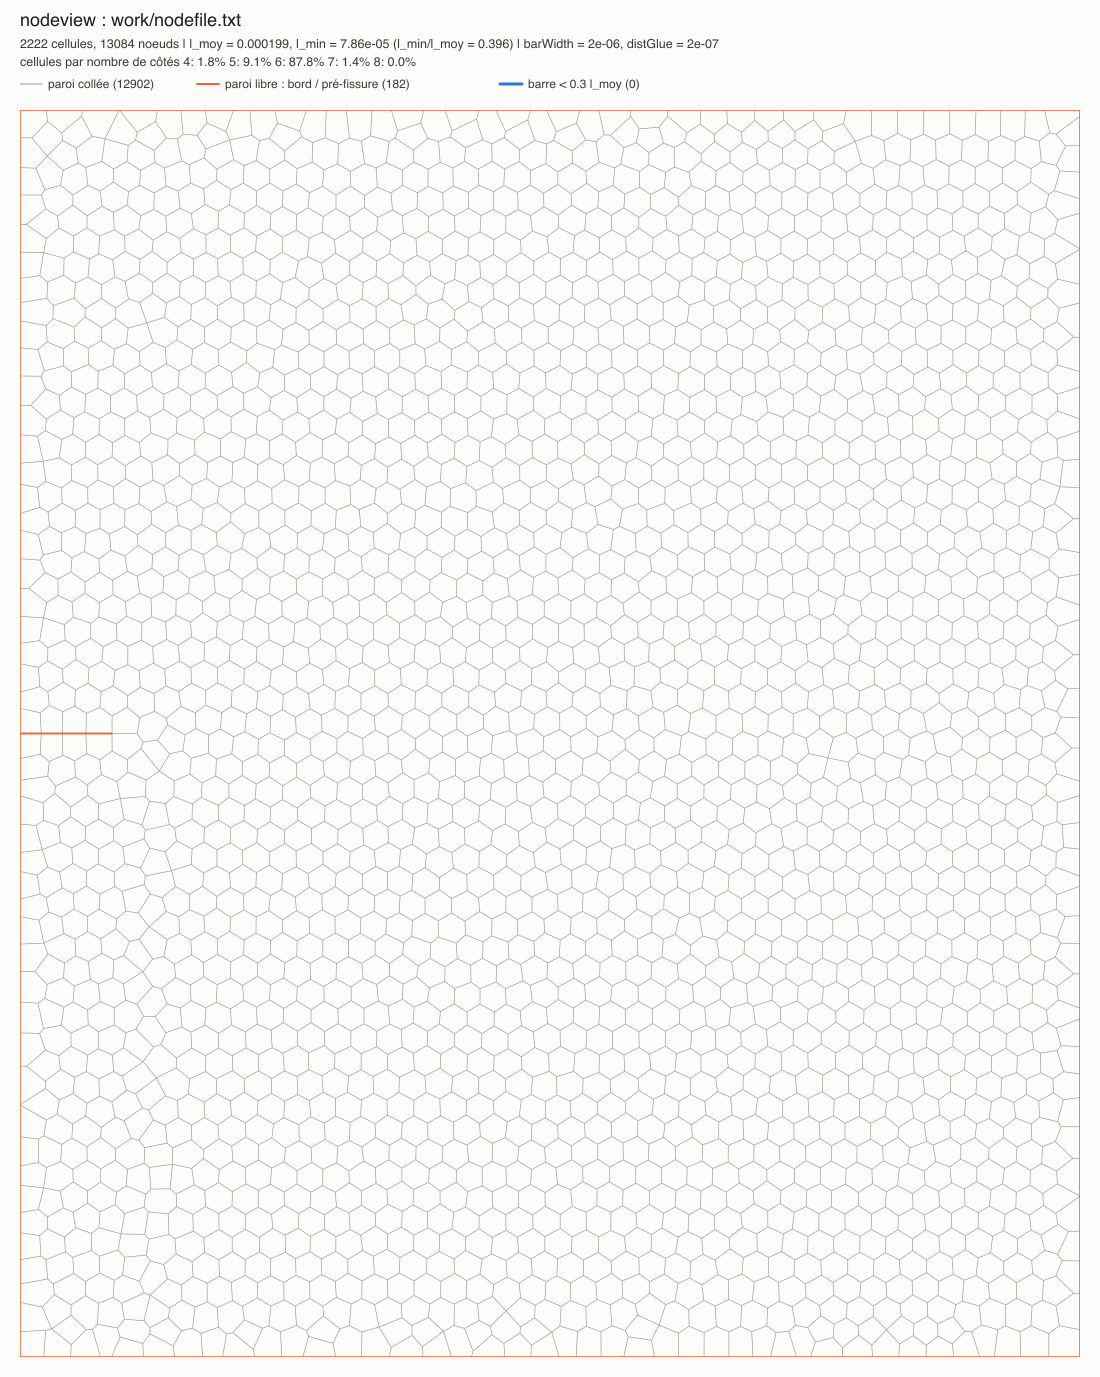
\includegraphics[width=0.62\linewidth]{figures/example_legend.png}
  \caption{Vue produite par \toolgen{} pour \code{tutorial\_params.txt}. En gris : parois collées ; en orange :
    parois libres (bords du domaine et pré-fissure) ; en bleu : barres courtes (aucune ici).}
  \label{fig:example}
\end{figure}

%======================================================================
\section{Paramètres}
%======================================================================

Le fichier de paramètres contient un mot-clé par ligne ; tout ce qui suit \code{\#} est un commentaire.

\begin{center}
\small
\begin{tabular}{@{}llp{9.6cm}@{}}
  \toprule
  Mot-clé & Défaut & Rôle \\
  \midrule
  \code{xmin}, \code{ymin} & 0, 0 & coin inférieur gauche du domaine \\
  \code{Lx}, \code{Ly} & 0.01 & dimensions du domaine \\
  \code{cellSize} & 3.5e-4 & diamètre équivalent visé ; le nombre de cellules vaut $L_xL_y/(\pi d^2/4)$ \\
  \code{barWidth} & 2e-6 & largeur des barres, à reporter dans \code{readNodeFile} \\
  \midrule
  \code{lattice} & \code{hex} & \code{hex} : réseau hexagonal perturbé ; \code{random} : tirage aléatoire \\
  \code{disorder} & 0.3 & perturbation des germes du réseau \code{hex} (fraction du pas) \\
  \code{lloydIterations} & 10 & itérations de régularisation de Lloyd \\
  \code{seed} & 1 & graine du générateur aléatoire \\
  \midrule
  \code{minEdgeRatio} & 0.3 & seuil des arêtes courtes, en fraction de la longueur moyenne \\
  \code{minSides} & 5 & une fusion d'arête ne peut faire passer une cellule sous \code{minSides} côtés ;
    sinon l'arête est étirée \\
  \midrule
  \code{crack x0 y0 x1 y1} & --- & pré-fissure (segment), facultative \\
  \code{opening} & 2e-6 & écart supplémentaire entre les lèvres de la fissure \\
  \code{tipInterface} & 1 & longueur (en cellules) de l'interface collée qui prolonge la fissure \\
  \code{distGlue} & 2e-7 & valeur de \code{distGcGlue} de l'input, pour les contrôles \\
  \midrule
  \code{cellProperties} & --- & \code{Kn Kr Mz\_max p\_int} reportés dans \code{readNodeFile} \\
  \code{glueProperties} & --- & \code{kn\_coh kt\_coh Gc} reportés dans \code{setGcGlueSameProperties} \\
  \code{gripRows} & 1 & nombre de rangées de nœuds attrapées par chacun des mors bas et haut \\
  \code{gripHeight} & --- & hauteur explicite des mors (si \code{gripRows} n'est pas donné) \\
  \code{pullVelocity} & 3e-4 & vitesse imposée aux mors (bas $-v$, haut $+v$) \\
  \code{nodeMass} & --- & masse des nœuds, pour estimer le pas de temps critique de flexion \\
  \midrule
  \code{inputTemplate} & --- & \code{modèle [sortie]} : input complet produit à partir d'un input existant
    (sortie par défaut \code{input.txt}) \\
  \code{output}, \code{svg}, \code{input} & & nodeFile, vue SVG, lignes d'input \textsc{l-hyphen} \\
  \bottomrule
\end{tabular}
\end{center}

\paragraph{Choisir la régularité.} \code{lattice} et \code{disorder} règlent la forme des cellules
(figure~\ref{fig:disorder}). Sur la géométrie du tutoriel, avec \code{lloydIterations 5} et \code{minSides 5}, on
obtient pour les cellules intérieures :

\begin{center}
\begin{tabular}{lcccc}
  \toprule
  Réglage & 4 côtés & 5 côtés & 6 côtés & 7 côtés \\
  \midrule
  \code{lattice random}, \code{lloydIterations 10} & \SI{0.3}{\%} & \SI{44}{\%} & \SI{47}{\%} & \SI{8}{\%} \\
  \code{lattice hex}, \code{disorder 0.2} & \SI{0.1}{\%} & \SI{4.5}{\%} & \SI{95}{\%} & \SI{0.4}{\%} \\
  \code{lattice hex}, \code{disorder 0.3} & \SI{0.1}{\%} & \SI{5}{\%} & \SI{94}{\%} & \SI{1.3}{\%} \\
  \code{lattice hex}, \code{disorder 0.4} & \SI{0}{\%} & \SI{16}{\%} & \SI{83}{\%} & \SI{0.8}{\%} \\
  \bottomrule
\end{tabular}
\end{center}

\begin{figure}[H]
  \centering
  \begin{subfigure}{0.32\linewidth}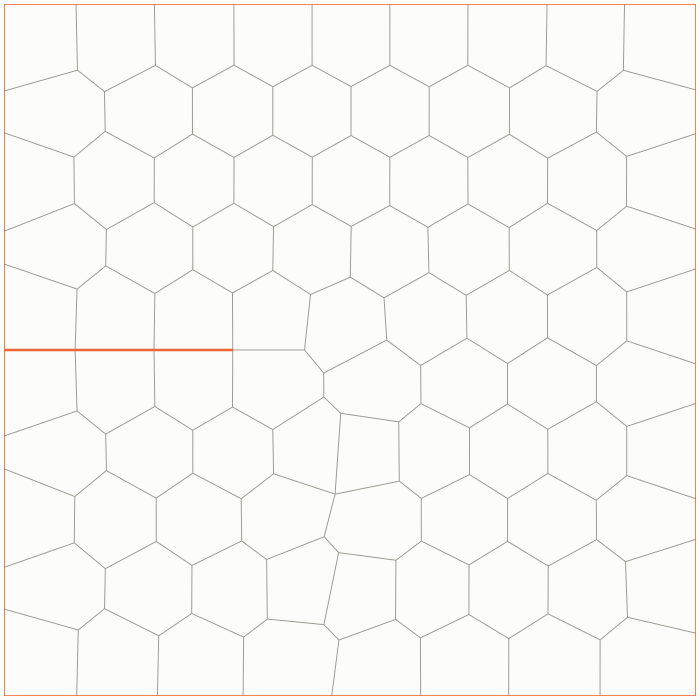
\includegraphics[width=\linewidth]{figures/disorder_0.png}\caption{\code{disorder 0}}\end{subfigure}\hfill
  \begin{subfigure}{0.32\linewidth}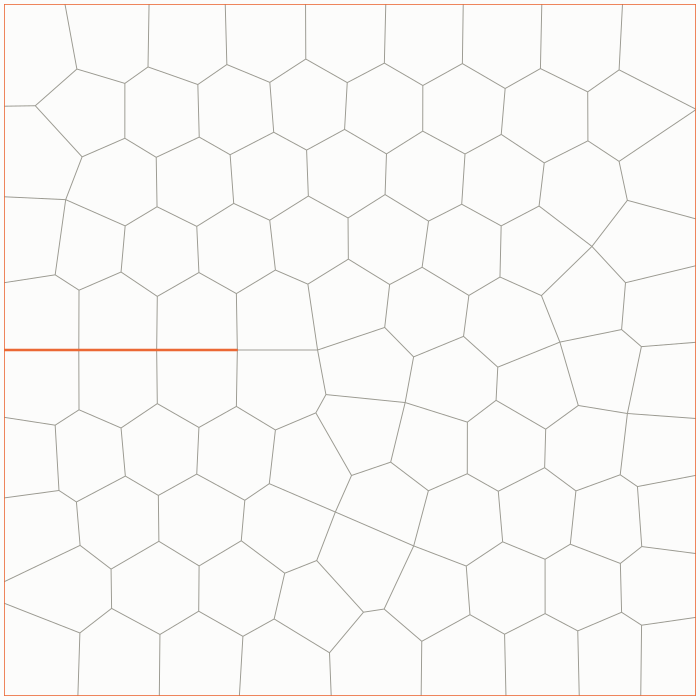
\includegraphics[width=\linewidth]{figures/disorder_0.3.png}\caption{\code{disorder 0.3}}\end{subfigure}\hfill
  \begin{subfigure}{0.32\linewidth}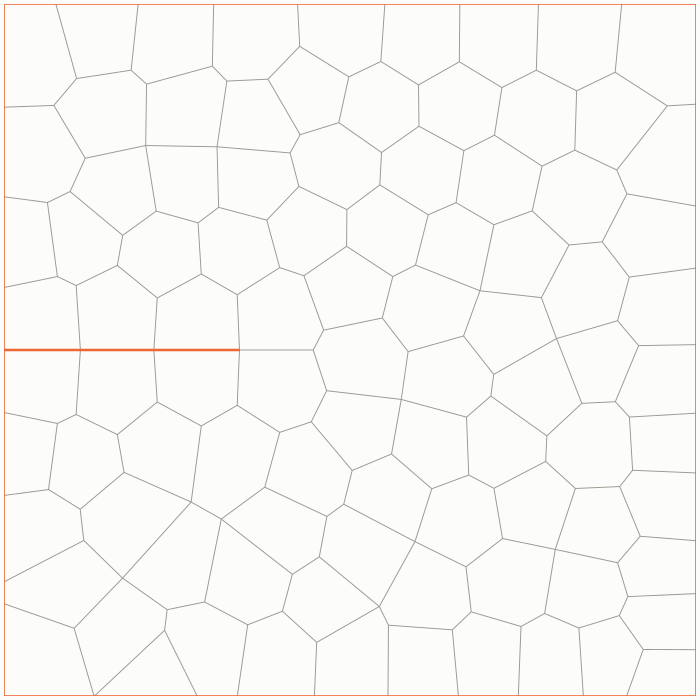
\includegraphics[width=\linewidth]{figures/disorder_0.5.png}\caption{\code{disorder 0.5}}\end{subfigure}
  \caption{Effet de \code{disorder} (réseau hexagonal, domaine de \SI{3}{mm}, pré-fissure de \SI{1}{mm}). Le long
    de la fissure, la rangée de cellules est symétrique ; plus loin, le réseau est régulier.}
  \label{fig:disorder}
\end{figure}

\paragraph{Pré-fissure.} Le segment \code{crack} peut partir d'un bord (fissure débouchante) ou être entièrement
intérieur, et avoir une orientation quelconque. \code{opening} doit être nettement supérieur à \code{distGlue}
pour que les lèvres ne soient pas collées. \code{tipInterface} fixe la longueur de l'interface collée qui prolonge
la fissure au-delà de la pointe (section~\ref{sec:tip}).

%======================================================================
\section{Visualiser et contrôler un nodeFile avec \toolview}
%======================================================================

\begin{lstlisting}
nodeview nodefile.txt [-w barWidth] [-g distGlue] [-r ratio] [-box x0 x1 y0 y1]
                      [-nodes] [-bare] [-px largeur] [-o out.svg]
\end{lstlisting}

\toolview{} lit n'importe quel nodeFile (y compris ceux de \code{cellPrepro}) comme \code{readNodeFile} le fait, et
produit un SVG (vectoriel : le zoom est illimité dans un navigateur). Chaque paroi est classée :
\begin{itemize}[nosep]
  \item \textcolor{glued}{\textbf{collée}} si son milieu est à moins de \code{barWidth + distGlue} d'une barre
    d'une autre cellule --- c'est le critère de création des liens cohésifs de \textsc{l-hyphen}, et le nombre de
    parois collées est égal au nombre de « liens collés » affiché par \code{diagnostic.txt} ;
  \item \textcolor{free}{\textbf{libre}} sinon : bord du domaine, pré-fissure, trou ;
  \item les barres plus courtes que \code{ratio} $\times\,\bar\ell$ (défaut 0.3) sont surlignées en
    \textcolor{short}{\textbf{bleu}}.
\end{itemize}
Sans \code{-w}, la largeur des barres est estimée par la distance minimale entre nœuds de cellules différentes.
\code{-box} restreint le dessin à une fenêtre (zoom), \code{-nodes} dessine les nœuds, \code{-bare} supprime
titre et légende.

\begin{figure}[H]
  \centering
  \begin{subfigure}{0.48\linewidth}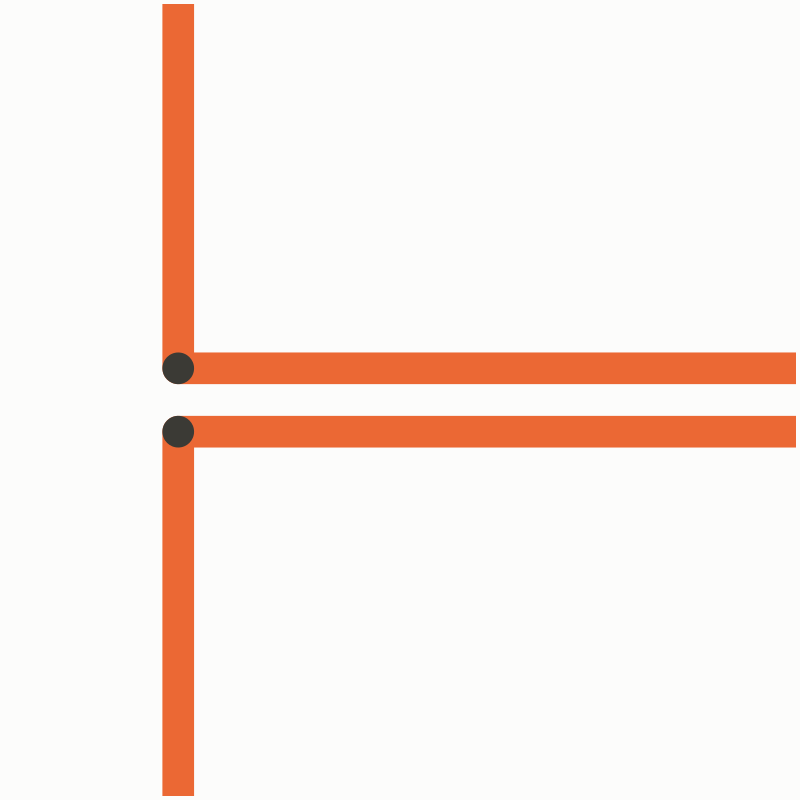
\includegraphics[width=\linewidth]{figures/example_mouth.png}
    \caption{Embouchure de la fissure (fenêtre de \SI{50}{\micro m})}\end{subfigure}\hfill
  \begin{subfigure}{0.48\linewidth}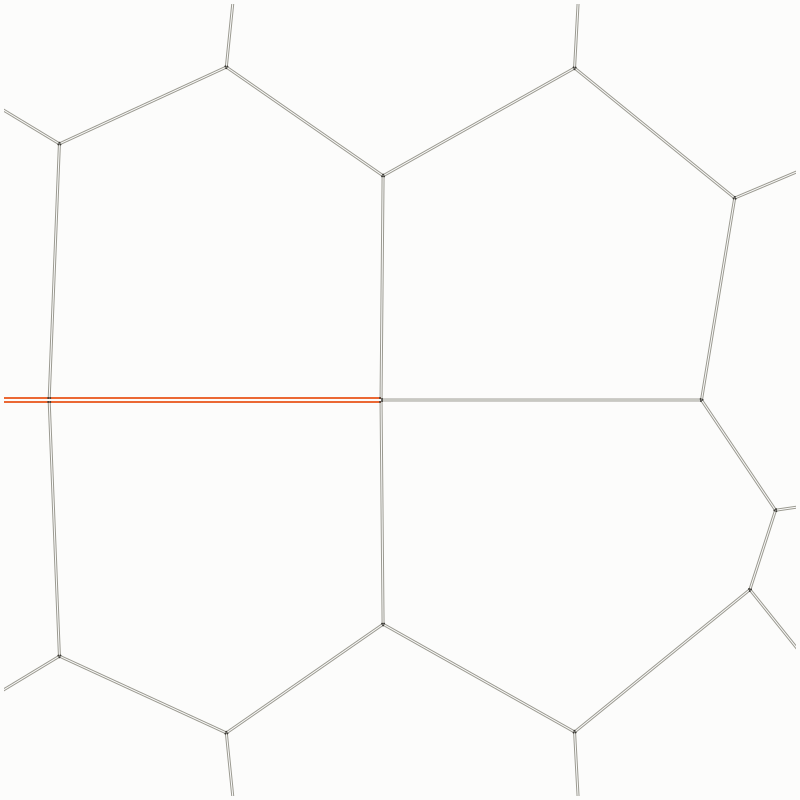
\includegraphics[width=\linewidth]{figures/example_tip.png}
    \caption{Pointe de la fissure (fenêtre de \SI{0.8}{mm})}\end{subfigure}
  \caption{Zooms obtenus avec \code{-box} et \code{-nodes}. (a) Les lèvres de la fissure sont écartées de
    \code{barWidth + opening} = \SI{4}{\micro m}, les parois collées de \code{barWidth} = \SI{2}{\micro m}.
    (b) La fissure se termine sur un sommet et se prolonge par une interface collée.}
  \label{fig:zoom}
\end{figure}

\begin{figure}[H]
  \centering
  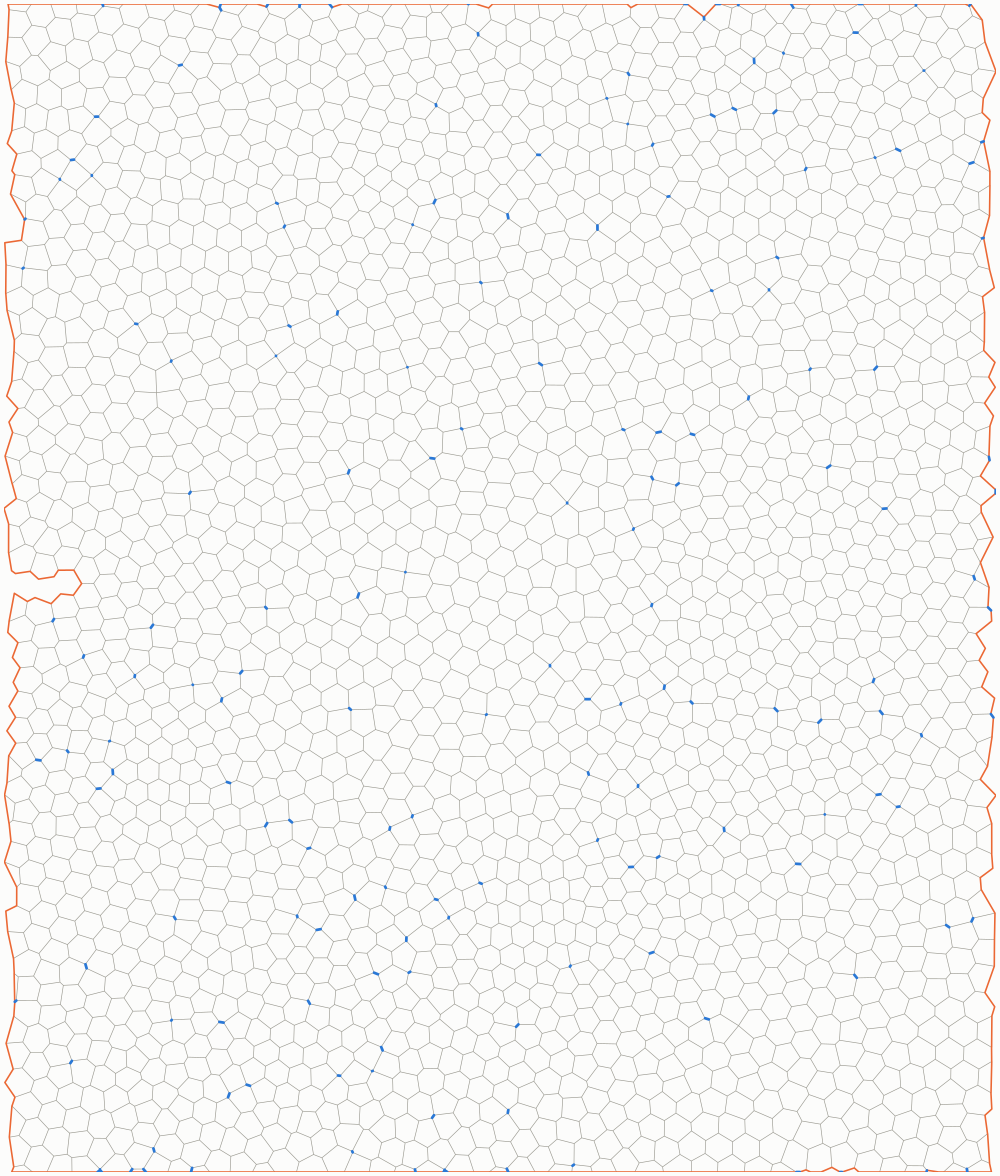
\includegraphics[width=0.55\linewidth]{figures/frank.png}
  \caption{\toolview{} appliqué au nodeFile de \code{Frank-ouverture-fissure} (produit par \code{cellPrepro}) :
    pré-fissure obtenue en retirant des cellules, bords latéraux irréguliers et 331 barres plus courtes que
    $0.3\,\bar\ell$ (en bleu), la plus courte mesurant $0.012\,\bar\ell$.}
  \label{fig:frank}
\end{figure}

%======================================================================
\section{Produire le fichier d'input \textsc{l-hyphen}}
\label{sec:input}

\subsection{Input complet à partir d'un modèle (\code{inputTemplate})}

Le plus simple est de partir d'un fichier d'input existant, par exemple celui d'une étude précédente :
\begin{lstlisting}
inputTemplate  modele_input.txt  work/input.txt
\end{lstlisting}
\toolgen{} recopie le modèle dans \code{work/input.txt} en remplaçant les lignes qui dépendent du maillage,
marquées \code{\# [nodegen]}. Tous les autres réglages du modèle (pas de temps, raideurs de contact, masses,
amortissements, sorties\dots) sont conservés, y compris les constantes \code{define} et les expressions.

\begin{center}
\small
\begin{tabular}{@{}lp{10.4cm}@{}}
  \toprule
  Ligne du modèle & Traitement \\
  \midrule
  \code{readNodeFile} & nouveau nodeFile (chemin relatif au répertoire de l'input produit) et \code{barWidth} ;
    \code{Kn Kr Mz\_max p\_int} de \code{cellProperties}, sinon recopiés du modèle \\
  \code{cleanShortBars} & commentée (inutile) \\
  2 \code{setNodeControlInBox} & boîtes recalculées sur le nouveau domaine, de hauteur fixée par \code{gripRows}
    (section~\ref{sec:grips}) ; modes et valeurs repris du modèle, sauf si \code{pullVelocity} est donné \\
  2 \code{captureNodes} & boîtes recalculées, noms de fichiers conservés \\
  \code{setGcGlueSameProperties} & remplacée si \code{glueProperties} est donné, sinon recopiée \\
  \code{distGcGlue}, \code{glue} & recopiée ; \toolgen{} vérifie qu'elle reste inférieure à \code{opening} \\
  autres lignes & recopiées telles quelles \\
  \bottomrule
\end{tabular}
\end{center}

Les mors bas et haut sont reconnus comme les deux boîtes de plus petit et de plus grand $y_{\min}$. Si le modèle ne
contient pas exactement deux \code{setNodeControlInBox} (ou deux \code{captureNodes}), ces lignes sont recopiées
sans modification et un avertissement est affiché. \toolgen{} affiche le nombre de nœuds de chaque mors et, si la
masse des nœuds et $k_r$ sont connus, le pas de temps critique de flexion ; il refuse d'écraser le modèle.

Différences entre le modèle (input de \code{Frank-ouverture-fissure}) et l'input produit pour le tutoriel :

\lstinputlisting[basicstyle=\ttfamily\scriptsize]{figures/deck_diff.txt}

L'input produit a été lancé sans autre modification que la durée simulée (\num{20000} pas) : aucune rupture au
démarrage et 12902 liens collés, comme attendu.

\subsection{Lignes d'input seules}
%======================================================================

Sans modèle, \toolgen{} écrit toujours dans le fichier \code{input} (défaut \code{nodegen\_input.txt}) les
lignes d'input qui dépendent du maillage, à copier dans un fichier d'input aux endroits indiqués :
\begin{itemize}[nosep]
  \item \code{readNodeFile} avec le bon \code{barWidth} et les propriétés de \code{cellProperties} ;
  \item les mors : deux \code{setNodeControlInBox} sur toute la largeur (section~\ref{sec:grips}), libres en $x$
    (mode 1, force nulle) et à vitesse imposée $\mp v$ en $y$ (mode 0), avec le nombre de nœuds de chaque mors,
    et les deux \code{captureNodes} correspondants ;
  \item \code{distGcGlue} et \code{setGcGlueSameProperties} (propriétés de \code{glueProperties}) ;
  \item en commentaire, les statistiques du maillage, la position effective de la pointe et, si \code{nodeMass}
    est donné, le pas de temps critique de flexion $\ell_{\min}\sqrt{m/k_r}$.
\end{itemize}
Une ligne dont une valeur n'est pas connue est écrite en commentaire, avec des repères \code{<...>} à compléter.
Pour \code{tutorial\_params.txt} :

\lstinputlisting[basicstyle=\ttfamily\scriptsize]{figures/nodegen_input.txt}

L'ordre compte : \code{readNodeFile} ouvre la section de l'échantillon (avant les masses et les amortissements),
les contrôles et \code{captureNodes} suivent, et le collage vient en dernier, une fois \code{distVerlet} défini.
Le nombre de nœuds de chaque mors permet de vérifier que la hauteur des mors est adaptée ; \toolgen{} signale un
mors vide ou une pré-fissure qui entrerait dans un mors.

\subsection{Mors : rangées de nœuds attrapées}
\label{sec:grips}

Les mors bas et haut sont deux boîtes \code{setNodeControlInBox} de toute la largeur du domaine. Par défaut
(\code{gripRows 1}), chacune attrape \textbf{une seule rangée de nœuds} : les nœuds du bord, tous situés à
\code{barWidth}/2 du bord du domaine. Les parois des cellules de bord restent alors libres de se déformer ; seuls
leurs nœuds sur le bord sont pilotés.

Les rangées sont définies topologiquement : la rangée~1 est formée des sommets du bord, la rangée~$k$ des sommets
situés à $k-1$ barres du bord (les nœuds des cellules voisines au même sommet comptant pour un seul sommet). Une
boîte ne sélectionne que par la hauteur ; \toolgen{} la fait s'arrêter à mi-distance entre le nœud le plus haut
des \code{gripRows} premières rangées et le nœud suivant. Sur l'échantillon du tutoriel :

\begin{center}
\begin{tabular}{lccc}
  \toprule
  Mors bas & hauteur de la boîte & nœuds attrapés & dont nœuds des rangées suivantes \\
  \midrule
  \code{gripRows 1} (défaut) & \SI{39}{\micro m} & 82 & 0 \\
  \code{gripRows 2} & \SI{354}{\micro m} & 253 & 45 \\
  \code{gripRows 3} & \SI{819}{\micro m} & 651 & 303 \\
  \code{gripHeight 4e-4} & \SI{400}{\micro m} & 312 & --- \\
  \bottomrule
\end{tabular}
\end{center}

La première rangée est attrapée exactement : le nœud suivant est à environ \SI{78}{\micro m} du bord. Au-delà,
un pavage de Voronoï n'a pas de rangées horizontales (le nœud le plus haut de la rangée~2 est plus haut que le
nœud le plus bas de la rangée~3) : la boîte attrape toutes les rangées demandées, plus quelques nœuds bas des
rangées suivantes, dont \toolgen{} affiche le nombre. \code{gripHeight} impose directement une hauteur de boîte.

\subsection{Vérifications}

\code{cleanShortBars} est inutile avec un nodeFile produit par \toolgen. Avec les mors d'une rangée, l'input du
tutoriel a été lancé sur \num{20000} pas : aucune rupture, et des forces égales et opposées sur les deux mors
(\SI{-1.405}{mN} en haut, \SI{1.403}{mN} en bas à $t=\SI{1}{ms}$). Après un premier lancement, vérifier dans
\code{diagnostic.txt} que le nombre de « liens collés » est égal au nombre de parois collées de \toolview, et que le
rapport $\Delta t_{\text{crit}}/\Delta t$ de la ligne « flexion » est confortable. Sur l'échantillon du tutoriel,
avec les paramètres mécaniques de \code{Frank-ouverture-fissure} :

\begin{center}
\begin{tabular}{lcc}
  \toprule
  & Frank (\code{cellPrepro}) & \toolgen{} (tutoriel) \\
  \midrule
  cellules / nœuds & 2155 / 12798 & 2222 / 13084 \\
  $\ell_{\min}/\bar\ell$ & 0.012 & 0.40 \\
  $\Delta t_{\text{crit,flexion}}$ & \SI{2.4e-8}{s} & \SI{7.9e-7}{s} \\
  liens collés (\code{diagnostic.txt}) & 12542 & 12902 \\
  ruptures au démarrage (\num{20000} pas) & --- & 0 \\
  \bottomrule
\end{tabular}
\end{center}

%======================================================================
\section{Algorithmes}
%======================================================================

\begin{figure}[H]
  \centering
  \begin{tikzpicture}[node distance=4mm and 5mm, every node/.style={font=\small},
      box/.style={draw=ink, rounded corners=2pt, fill=gray!6, align=center, minimum height=12mm, text width=27mm},
      >={Stealth[length=2mm]}]
    \node[box] (s) {1. Germes\\\footnotesize réseau hex / aléatoire};
    \node[box, right=of s] (sym) {2. Symétrie\\\footnotesize autour de la fissure};
    \node[box, right=of sym] (l) {3. Lloyd\\\footnotesize (+ symétrie)};
    \node[box, right=of l] (v) {4. Voronoï\\\footnotesize demi-plans};
    \node[below=1mm of l, font=\footnotesize] {répété \code{lloydIterations} fois};
    \node[box, below=10mm of v] (t) {5. Sommets\\\footnotesize partagés, types};
    \node[box, left=of t] (e) {6. Arêtes courtes\\\footnotesize fusion/étirement};
    \node[box, left=of e] (o) {7. Décalage\\\footnotesize des parois};
    \node[box, left=of o] (w) {8. nodeFile\\\footnotesize + SVG};
    \draw[->] (s) -- (sym); \draw[->] (sym) -- (l); \draw[->] (l) -- (v); \draw[->] (v) -- (t);
    \draw[->] (t) -- (e); \draw[->] (e) -- (o); \draw[->] (o) -- (w);
  \end{tikzpicture}
  \caption{Chaîne de traitement de \toolgen.}
  \label{fig:pipeline}
\end{figure}

\begin{figure}[H]
  \centering
  \begin{subfigure}{0.32\linewidth}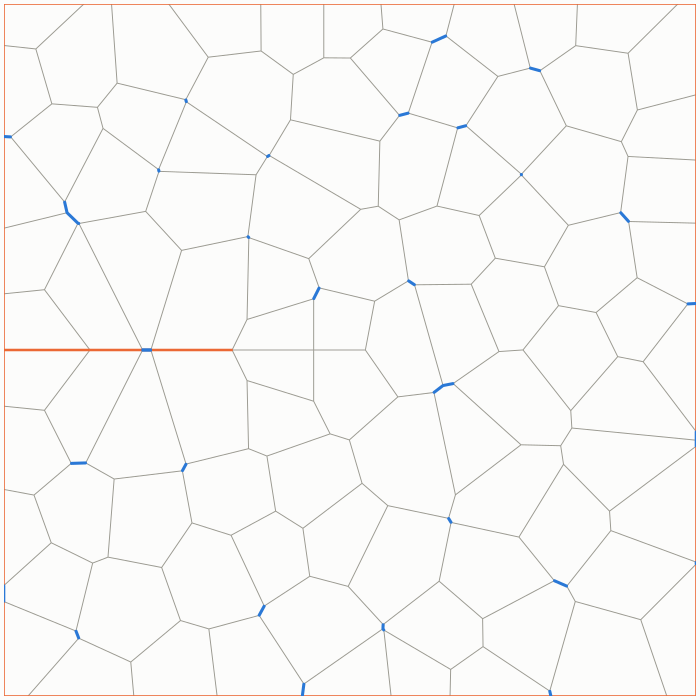
\includegraphics[width=\linewidth]{figures/stage_raw.png}
    \caption{Voronoï brut}\end{subfigure}\hfill
  \begin{subfigure}{0.32\linewidth}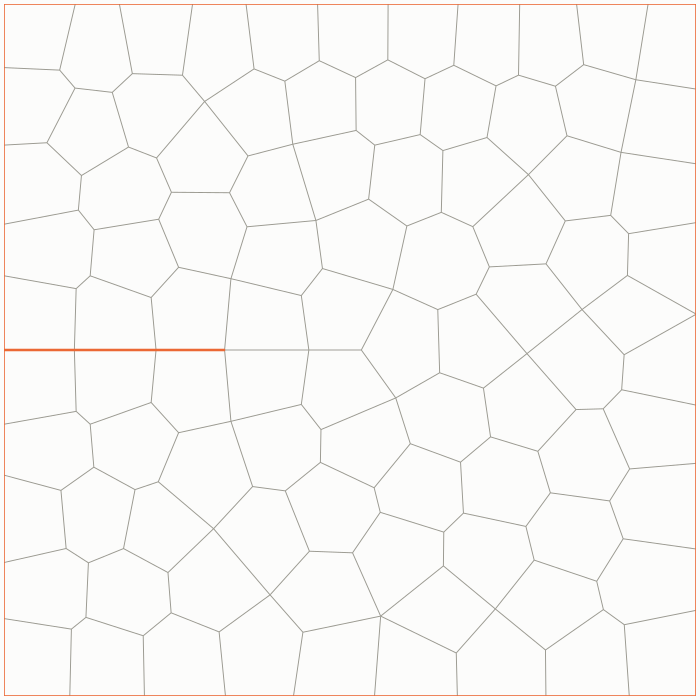
\includegraphics[width=\linewidth]{figures/stage_lloyd.png}
    \caption{Lloyd + fusion seule}\end{subfigure}\hfill
  \begin{subfigure}{0.32\linewidth}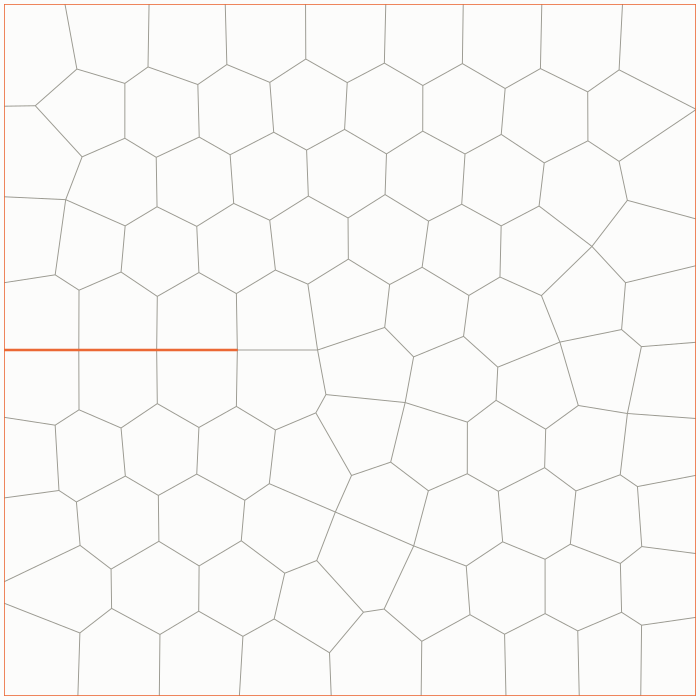
\includegraphics[width=\linewidth]{figures/stage_hex.png}
    \caption{Réseau hex + \code{minSides 5}}\end{subfigure}
  \caption{Trois réglages sur un domaine de \SI{3}{mm}. (a) Germes aléatoires, sans Lloyd ni traitement des
    arêtes courtes : nombreuses barres courtes (bleu), $\ell_{\min}=0.01\,\bar\ell$ et \SI{29}{\%} d'heptagones.
    (b) Lloyd (10 itérations) et fusion seule : $\ell_{\min}=0.34\,\bar\ell$, mais la fusion multiplie les pentagones
    (\SI{56}{\%}). (c) Réseau hexagonal, \code{disorder 0.3}, fusion limitée par \code{minSides 5} et étirement :
    $\ell_{\min}=0.40\,\bar\ell$, uniquement des pentagones et des hexagones.}
  \label{fig:stages}
\end{figure}

\subsection{Germes}

\paragraph{Tirage aléatoire (\code{lattice random}).} On vise $N = L_xL_y/A$ cellules d'aire
$A=\pi d^2/4$ ($d$ = \code{cellSize}), d'espacement moyen $s=\sqrt{A}$. Les germes sont tirés uniformément et
acceptés s'ils sont à plus de $r_{\min}=0.7\,s$ des germes déjà placés (recherche par grille) ; si la saturation
est atteinte avant $N$, le complément est tiré sans contrainte.

\paragraph{Réseau hexagonal (\code{lattice hex}).} Un réseau triangulaire de germes, de pas
$a=\sqrt{2A/\sqrt3}$ (aire de la cellule hexagonale égale à $A$) et d'interrangée $a\sqrt3/2$, donne un pavage
d'hexagones réguliers. Chaque germe est ensuite déplacé d'un vecteur aléatoire uniforme dans un disque de rayon
\code{disorder}~$\times\,a$. Le réseau est exprimé dans le repère de la fissure $(\mathbf t,\mathbf n)$ (rangées
parallèles à la fissure) et décalé pour qu'un sommet du réseau tombe sur la pointe. Le long de la fissure, les
rangées sont placées symétriquement de part et d'autre de la ligne (section~\ref{sec:crack}) ; ailleurs, elles
alternent normalement.

\subsection{Régularisation de Lloyd}

À chaque itération, le pavage de Voronoï est calculé et chaque germe est déplacé au centroïde de sa cellule :
\[
  \mathbf x_i \leftarrow \frac{1}{|\Omega_i|}\int_{\Omega_i}\mathbf x\,\mathrm dA .
\]
Les itérations tendent vers un pavage de Voronoï centroïdal, aux cellules d'aires voisines et majoritairement
hexagonales. La symétrie autour de la fissure est rétablie après chaque itération.

\subsection{Pavage de Voronoï par découpe de demi-plans}

La cellule du germe $\mathbf p$ est l'intersection du rectangle et des demi-plans
$\{\mathbf x : (\mathbf x-\mathbf m)\cdot(\mathbf q-\mathbf p)\le 0\}$, $\mathbf m=(\mathbf p+\mathbf q)/2$, pour
tous les autres germes $\mathbf q$. Le polygone convexe est découpé successivement (algorithme de
Sutherland--Hodgman) par les germes des anneaux de grille de rang $k=0,1,2,\dots$ autour de $\mathbf p$ (pas de
grille $h=s$). Après l'anneau $k$, les germes restants sont à plus de $kh$ ; un germe à la distance $D$ ne
découpe la cellule que si $D<2R$, où $R$ est la distance de $\mathbf p$ au sommet le plus éloigné : on s'arrête
dès que $kh\ge2R$. Le coût est $O(N)$ pour une densité uniforme.

\subsection{Sommets partagés et types de sommets}

Chaque cellule est calculée indépendamment ; les sommets communs sont identifiés à $10^{-8}s$ près (table de
hachage spatiale), ce qui donne une topologie cohérente : chaque arête est partagée par deux cellules (ou bordée
par le domaine). Chaque sommet reçoit un type : bord gauche, droit, bas, haut, ligne de fissure, ou une
combinaison (coin, embouchure de la fissure).

\subsection{Arêtes courtes : fusion ou étirement}

Les arêtes plus courtes que $\ell_c=$ \code{minEdgeRatio}~$\times\,\bar\ell$ sont traitées de la plus courte à
la plus longue (figure~\ref{fig:merge}).

\begin{figure}[H]
  \centering
  \begin{tikzpicture}[scale=1.15, >={Stealth[length=2mm]}, font=\small]
    \begin{scope}
      \coordinate (u) at (0,0); \coordinate (v) at (0.45,0);
      \draw[ink, thick] (u) -- (v);
      \draw[ink] (u) -- ++(-1,0.9) (u) -- ++(-1,-0.9) (v) -- ++(1,0.9) (v) -- ++(1,-0.9);
      \fill (u) circle (1.3pt) node[left=3pt] {$u$}; \fill (v) circle (1.3pt) node[right=3pt] {$v$};
      \node at (0.22,0.8) {$A$}; \node at (0.22,-0.8) {$B$}; \node at (-1,0) {$C$}; \node at (1.45,0) {$D$};
      \node[below=12mm] at (0.22,0) {arête courte $uv$};
    \end{scope}
    \begin{scope}[xshift=4.3cm]
      \coordinate (m) at (0.22,0);
      \draw[ink] (m) -- ++(-1.2,0.9) (m) -- ++(-1.2,-0.9) (m) -- ++(1.2,0.9) (m) -- ++(1.2,-0.9);
      \fill (m) circle (1.5pt) node[above=3pt] {$M$};
      \node at (0.22,0.8) {$A$}; \node at (0.22,-0.8) {$B$}; \node at (-0.9,0) {$C$}; \node at (1.35,0) {$D$};
      \node[below=12mm,align=center] at (0.22,0) {fusion : $A$ et $B$ perdent\\un côté};
    \end{scope}
    \begin{scope}[xshift=8.6cm]
      \coordinate (u) at (-0.35,0); \coordinate (v) at (0.8,0);
      \draw[ink, thick] (u) -- (v);
      \draw[ink] (u) -- ++(-0.65,0.9) (u) -- ++(-0.65,-0.9) (v) -- ++(0.65,0.9) (v) -- ++(0.65,-0.9);
      \fill (u) circle (1.3pt); \fill (v) circle (1.3pt);
      \draw[->, short, thick] (0,0.12) -- (-0.33,0.12); \draw[->, short, thick] (0.45,0.12) -- (0.78,0.12);
      \node at (0.22,0.8) {$A$}; \node at (0.22,-0.8) {$B$}; \node at (-1,0) {$C$}; \node at (1.45,0) {$D$};
      \node[below=12mm,align=center] at (0.22,0) {étirement : la topologie\\est conservée};
    \end{scope}
  \end{tikzpicture}
  \caption{Traitement d'une arête courte $uv$ bordée par les cellules $A$ et $B$.}
  \label{fig:merge}
\end{figure}

\paragraph{Fusion.} Les deux sommets sont réunis (union-find sur les sommets partagés, donc pour toutes les
cellules à la fois). Les cellules $A$ et $B$ qui bordaient l'arête perdent un côté, $C$ et $D$ se touchent en
un point. La fusion est refusée si une cellule concernée passait sous \code{minSides} côtés (et jamais sous 3).
La position du sommet fusionné respecte les contraintes : un coin ou l'embouchure de la fissure reste fixe, un
sommet de bord ou de fissure reste sur sa ligne (moyenne des sommets contraints de même type), sinon le sommet
est placé au barycentre.

\paragraph{Étirement.} Si la fusion est refusée, les deux sommets sont écartés le long de l'arête,
$\mathbf u \leftarrow \mathbf u - \tfrac{\delta}{2}\mathbf e$, $\mathbf v \leftarrow \mathbf v + \tfrac{\delta}{2}\mathbf e$,
avec $\mathbf e$ la direction de l'arête et $\delta=\ell_c-\ell$. Un sommet contraint ne se déplace que le long de
sa ligne (projection), un coin ne bouge pas (l'autre sommet fait alors tout le chemin). Le déplacement est annulé
s'il rendait une cellule voisine non convexe. Jusqu'à 20 passes sont effectuées ; les arêtes qui restent trop
courtes sont signalées.

\paragraph{Pourquoi \code{minSides}.} La fusion seule réduit systématiquement le nombre de côtés des deux cellules
voisines de l'arête : sur un pavage aléatoire régularisé, elle produit \SI{6}{\%} de quadrilatères et \SI{45}{\%}
de pentagones. Avec \code{minSides 5}, les fusions qui créeraient des quadrilatères sont remplacées par des
étirements.

\subsection{Pré-fissure par symétrie}
\label{sec:crack}

\begin{figure}[H]
  \centering
  \begin{tikzpicture}[scale=1.1, >={Stealth[length=2mm]}, font=\small]
    \draw[free, very thick] (-3.2,0) -- (0.6,0);
    \draw[ink, thick] (0.6,0) -- (2.0,0);
    \draw[ink, dashed] (2.0,0) -- (3.5,0) node[right] {ligne};
    \foreach \x in {-2.6,-1.3,0} {
      \fill[short] (\x,0.62) circle (2pt); \fill[short] (\x,-0.62) circle (2pt);
      \draw[short!60, densely dotted] (\x,0.62) -- (\x,-0.62);
    }
    \fill[short] (1.3,0.62) circle (2pt); \fill[short] (1.3,-0.62) circle (2pt);
    \draw[short!60, densely dotted] (1.3,0.62) -- (1.3,-0.62);
    \node[short, above] at (-2.6,0.68) {$\mathbf p$}; \node[short, below] at (-2.6,-0.68) {$\mathbf p'$};
    \foreach \x in {-1.95,-0.65,0.6,1.95} { \fill (\x,0) circle (1.4pt); \draw[ink] (\x,0) -- ++(0,0.9) (\x,0) -- ++(0,-0.9); }
    \node[free, left] at (-3.2,0) {fissure};
    \node[below right=1pt] at (0.6,0) {pointe};
    \node[above=3pt, align=center] at (1.3,0.95) {interface\\collée};
    \draw[<->] (2.4,0.1) -- (2.4,0.55) node[midway,right] {$n$};
    \draw[|<->|] (-3.2,-1.3) -- (2.0,-1.3) node[midway,below] {bande symétrique, jusqu'à $L+$\code{tipInterface}};
  \end{tikzpicture}
  \caption{Germes symétriques par rapport à la ligne de fissure : la médiatrice de $\mathbf p$ et de son
    symétrique $\mathbf p'$ est la ligne elle-même, qui est donc formée d'arêtes du pavage. La fissure est ouverte
    jusqu'à la pointe ; au-delà, la ligne se prolonge par une interface collée.}
  \label{fig:mirror}
\end{figure}

Dans une bande de demi-largeur $2s$ autour de la fissure, les germes du côté $n<0$ sont supprimés et ceux du côté
$n\ge0$ sont dupliqués par symétrie. Un point $\mathbf x$ de la ligne est équidistant d'un germe et de son
symétrique ; si les germes les plus proches de $\mathbf x$ sont tous dans la bande, l'ensemble des germes les plus
proches est symétrique, et $\mathbf x$ est sur le bord de deux cellules symétriques. La ligne est donc exactement
une suite d'arêtes du pavage : la fissure est rectiligne, aucune cellule n'est coupée ni retirée. Les germes trop
proches de la ligne ($n<r_{\min}/2$) sont repoussés à $n=r_{\min}/2$ pour éviter des cellules très aplaties.

\paragraph{Ouverture.} Le long de la fissure, les parois sont décalées de $w/2+o/2$ au lieu de $w/2$
($w$ = \code{barWidth}, $o$ = \code{opening}) : l'écart entre les lèvres vaut $w+o>w+$\code{distGlue}, donc aucun
lien cohésif n'y est créé (figure~\ref{fig:zoom}a).

\subsection{Pointe de fissure}
\label{sec:tip}

La bande symétrique est prolongée au-delà de la pointe : la ligne se continue par une interface \emph{collée}
entre deux cellules, et la pointe est un sommet où se rejoignent quatre cellules, en face d'une interface plutôt
que contre une cellule (figure~\ref{fig:zoom}b). La pointe est le sommet de la ligne le plus proche de
$(x_1,y_1)$ ; sa position effective est affichée.

Une ligne droite d'arêtes n'existe pas dans un pavage hexagonal : la rangée de pentagones qui borde la ligne doit se
raccorder au réseau régulier, ce qui crée un défaut (quelques pentagones et heptagones) au bout de l'interface.
\code{tipInterface} fixe la longueur de l'interface, donc la distance entre la pointe et ce défaut
(figure~\ref{fig:tip}). Au-delà, le réseau est régulier, afin de ne pas prolonger la fissure par une interface
rectiligne qui serait un chemin de rupture privilégié.

\begin{figure}[H]
  \centering
  \begin{subfigure}{0.32\linewidth}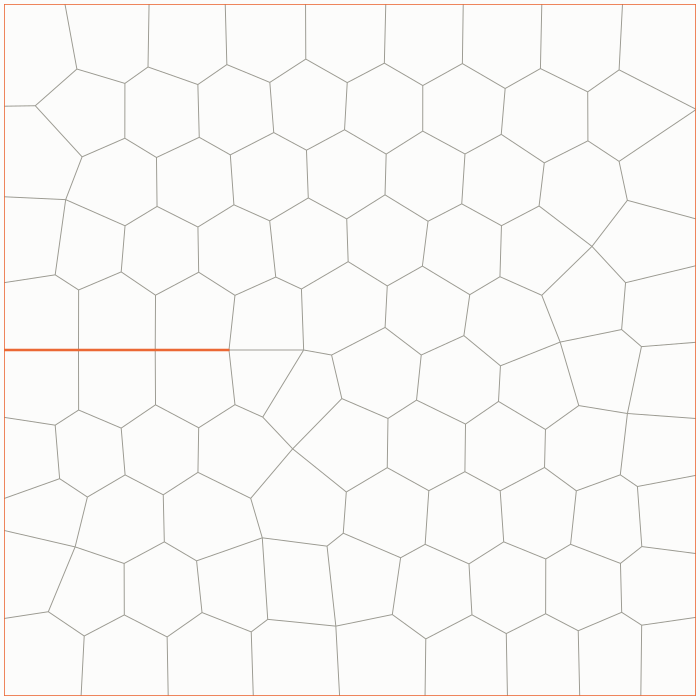
\includegraphics[width=\linewidth]{figures/tip_0.png}\caption{\code{tipInterface 0}}\end{subfigure}\hfill
  \begin{subfigure}{0.32\linewidth}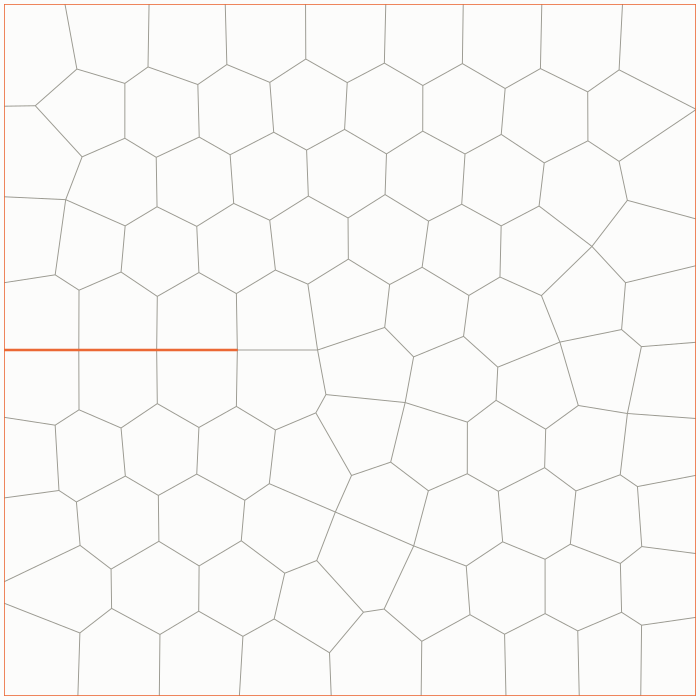
\includegraphics[width=\linewidth]{figures/tip_1.png}\caption{\code{tipInterface 1}}\end{subfigure}\hfill
  \begin{subfigure}{0.32\linewidth}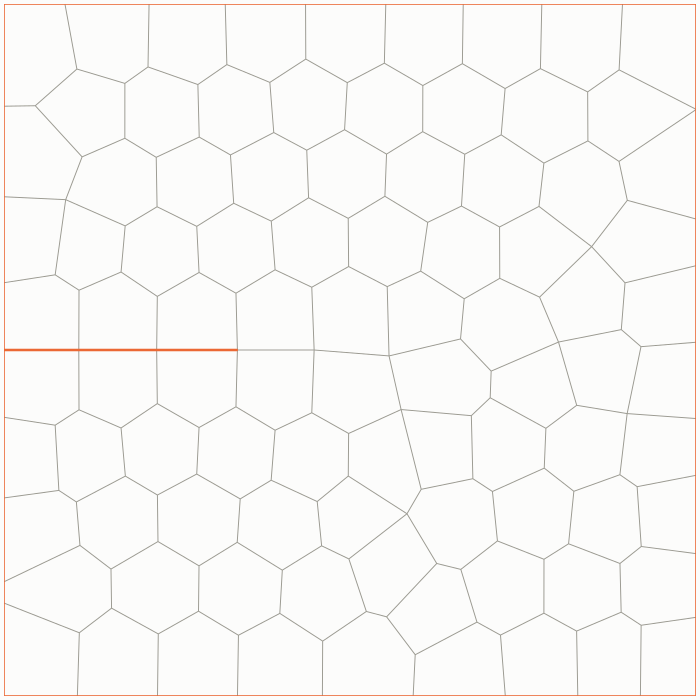
\includegraphics[width=\linewidth]{figures/tip_2.png}\caption{\code{tipInterface 2}}\end{subfigure}
  \caption{Longueur de l'interface collée qui prolonge la fissure (en orange) au-delà de la pointe.}
  \label{fig:tip}
\end{figure}

\subsection{Décalage des parois}

\begin{figure}[H]
  \centering
  \begin{tikzpicture}[scale=1.5, >={Stealth[length=2mm]}, font=\small]
    \coordinate (A) at (-2.4,0.35); \coordinate (P) at (0,0); \coordinate (B) at (1.1,1.7);
    % côtés décalés vers l'intérieur (à gauche du parcours A -> P -> B)
    \coordinate (A1) at ($(A)!0.42cm!90:(P)$);  \coordinate (P1) at ($(P)!0.42cm!-90:(A)$);
    \coordinate (P2) at ($(P)!0.30cm!90:(B)$);  \coordinate (B2) at ($(B)!0.30cm!-90:(P)$);
    \coordinate (S) at (intersection of A1--P1 and P2--B2);
    \draw[ink, very thick] (A) -- (P) -- (B);
    \draw[ink, dashed] ($(A1)!-0.05!(P1)$) -- ($(A1)!1.25!(P1)$);
    \draw[ink, dashed] ($(B2)!-0.05!(P2)$) -- ($(B2)!1.35!(P2)$);
    \draw[<->] ($(A)!0.45!(P)$) -- ($(A1)!0.45!(P1)$) node[midway,left] {$h_1$};
    \draw[<->] ($(P)!0.6!(B)$) -- ($(P2)!0.6!(B2)$) node[midway,above left=-1pt] {$h_2$};
    \fill (P) circle (1.4pt) node[below right] {$\mathbf P$ (sommet du pavage)};
    \fill[short] (S) circle (1.7pt);
    \node[short, above left] at (S) {$\mathbf S$ (nœud)};
    \node[ink] at (-1.3,1.25) {intérieur de la cellule};
  \end{tikzpicture}
  \caption{Le nœud $\mathbf S$ est l'intersection des deux côtés adjacents décalés vers l'intérieur de $h_1$ et
    $h_2$ ($w/2$, ou $w/2+o/2$ le long de la fissure).}
  \label{fig:inset}
\end{figure}

Chaque cellule (polygone convexe orienté dans le sens direct) est rétrécie en décalant chacun de ses côtés vers
l'intérieur : de $h=w/2$ en général, de $h=w/2+o/2$ pour un côté de la fissure. Pour un sommet $\mathbf P$ entre
deux côtés de normales intérieures unitaires $\mathbf n_1$, $\mathbf n_2$, le nœud $\mathbf S$ vérifie
\[
  \mathbf n_1\cdot\mathbf S = \mathbf n_1\cdot\mathbf P + h_1, \qquad
  \mathbf n_2\cdot\mathbf S = \mathbf n_2\cdot\mathbf P + h_2 ,
\]
système $2\times2$ résolu directement (si les deux côtés sont alignés, $\mathbf S=\mathbf P+\min(h_1,h_2)\,\mathbf n_1$).
C'est la construction de \code{cellPrepro}. Deux cellules voisines décalent la \emph{même} droite (le côté
commun) de part et d'autre : leurs parois sont exactement à la distance $w$, condition de création des liens
cohésifs par \code{glue} / \code{distGcGlue}. On vérifie enfin qu'aucun côté n'a été retourné par le décalage.

%======================================================================
\section{Validation sur un essai d'ouverture}
%======================================================================

Le nodeFile du tutoriel a été utilisé à la place de celui de \code{Frank-ouverture-fissure}, avec le même
fichier d'input (sans \code{cleanShortBars}), ainsi qu'un nodeFile produit par une première version de \toolgen{}
(germes aléatoires, fusion seule, fissure butant sur une cellule).

\begin{figure}[H]
  \centering
  \begin{subfigure}{0.48\linewidth}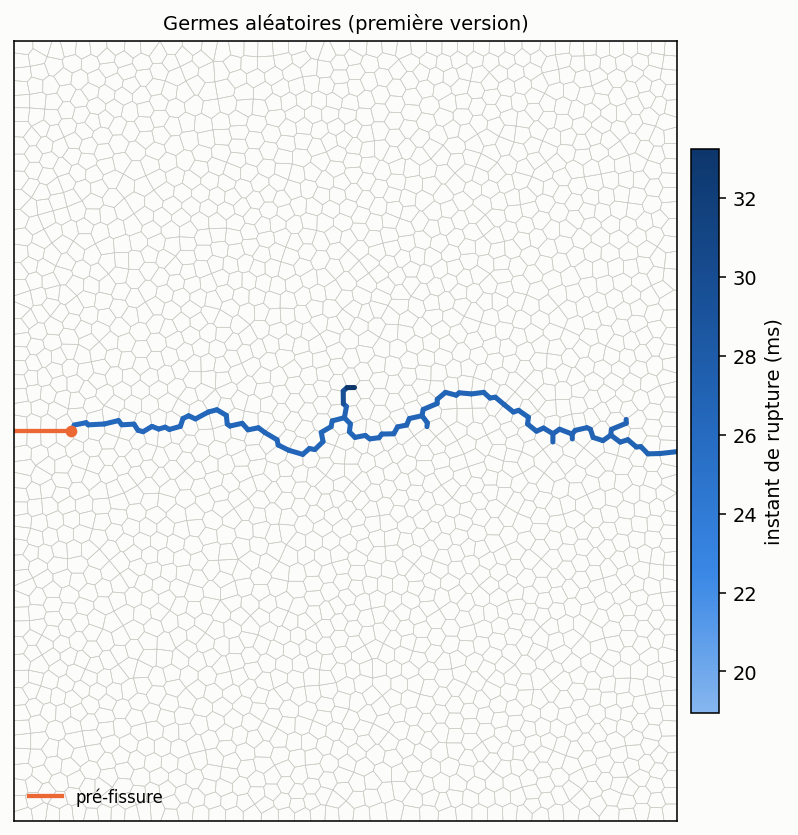
\includegraphics[width=\linewidth]{figures/crack_random.png}
    \caption{Germes aléatoires (première version)}\end{subfigure}\hfill
  \begin{subfigure}{0.48\linewidth}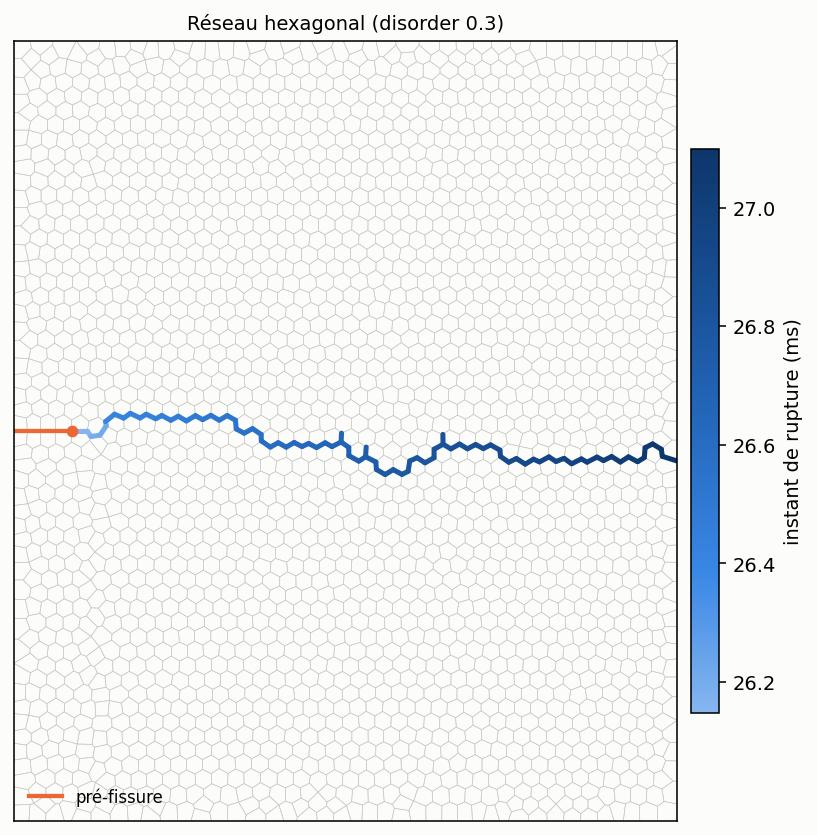
\includegraphics[width=\linewidth]{figures/crack_hex.png}
    \caption{Réseau hexagonal (\code{tutorial\_params.txt})}\end{subfigure}
  \caption{Chemins de fissuration obtenus avec \textsc{l-hyphen} (liens rompus, colorés selon l'instant de
    rupture ; en orange, la pré-fissure).}
  \label{fig:crack}
\end{figure}

% Résultats des calculs de validation (input de Frank-ouverture-fissure, dt = 5e-8 s, 0.045 s simulées)
\begin{center}
\begin{tabular}{lccc}
  \toprule
  & Frank (\code{cellPrepro}) & \toolgen{} aléatoire & \toolgen{} hexagonal \\
  \midrule
  force au pic (\si{mN}) & \num{-44.6} & \num{-44.2} & \num{-41.8} \\
  ouverture au pic (\si{\micro m}) & \num{17.6} & \num{15.7} & \num{15.6} \\
  première rupture (\si{ms}) & \num{29.33} & \num{18.94} (isolée), puis \num{26.21} & \num{26.15} \\
  fin de la propagation (\si{ms}) & \num{36.59} & \num{33.25} & \num{27.10} \\
  ruptures & 141 & 94 & 86 \\
  énergie rompue (\si{\micro J}) & 177 & 119 & 109 \\
  longueur rompue (\si{mm}) & \num{25.9} & \num{17.4} & \num{16.3} \\
  \bottomrule
\end{tabular}
\end{center}

La référence « Frank » est le calcul sur le nodeFile de \code{cellPrepro} au pas $\Delta t=\SI{1.75e-8}{s}$ ; les
deux maillages \toolgen{} sont calculés à $\Delta t=\SI{5e-8}{s}$ sans aucun nettoyage, avec l'amortissement de flexion
$\alpha_b=0.1$. Les maillages et les pré-fissures n'étant pas identiques, seule une comparaison qualitative a du
sens :
\begin{itemize}[nosep]
  \item avec les deux maillages \toolgen, la rupture s'amorce à la pointe de la pré-fissure ; avec le réseau hexagonal,
    les premiers liens rompus sont ceux de l'interface qui prolonge la fissure (à \SI{0.16}{mm} puis
    \SI{0.36}{mm} de la pointe) ;
  \item la fissure traverse l'échantillon en un seul chemin, sans bifurcation ; elle est sinueuse avec les germes
    aléatoires, mais suit en zigzag une rangée du réseau hexagonal et traverse l'échantillon en moins de
    \SI{1}{ms} : c'est l'anisotropie discutée à la section suivante ;
  \item le chemin plus direct explique l'énergie et la longueur rompues plus faibles qu'avec le maillage de Frank,
    dont la fissure bifurque.
\end{itemize}


%======================================================================
\section{Limites et améliorations possibles}
%======================================================================

\subsection{Anisotropie du réseau hexagonal}

Avec \code{lattice hex}, les rangées du réseau sont parallèles à la fissure : la fissure se propage en zigzag le
long d'une rangée (figure~\ref{fig:crack}b), ce qui est un artefact de l'ordre du réseau. Pistes :
\begin{itemize}[nosep]
  \item augmenter \code{disorder} (0.4--0.5), au prix de davantage de pentagones et d'heptagones ;
  \item orienter le réseau hors de la zone de la fissure selon un angle différent (par exemple \ang{30}, ou un
    angle aléatoire par « grain »), les raccords formant des joints de grains ;
  \item partir de germes aléatoires (isotropes) et contrôler le nombre de côtés par une optimisation
    topologique (paragraphe suivant) plutôt que par un réseau.
\end{itemize}

\subsection{Contrôle du nombre de côtés}

Le nombre de côtés n'est contrôlé qu'indirectement (réseau, \code{minSides}). Une optimisation explicite est
possible : transitions T1 (rotation d'une arête courte, qui retire un côté à deux cellules et en ajoute un aux
deux autres) choisies pour rapprocher chaque cellule de 5--6 côtés, ou pavage de puissance (Voronoï pondéré),
dont les poids permettent d'agrandir les cellules à trop peu de côtés et de réduire les autres (loi de Lewis :
l'aire d'une cellule croît avec son nombre de côtés).

\subsection{Géométrie}

\begin{itemize}[nosep]
  \item \textbf{Bords.} Les cellules de bord sont coupées par le rectangle (d'où les quadrilatères). Placer des
    germes symétriques par rapport aux bords donnerait des cellules de bord complètes et des bords rectilignes
    formés d'arêtes du pavage, comme pour la fissure.
  \item \textbf{Position exacte de la pointe.} La pointe est le sommet le plus proche du point demandé (à moins
    d'une demi-cellule) ; on pourrait ajuster le pas du réseau le long de la fissure pour qu'un sommet tombe
    exactement sur $(x_1,y_1)$.
  \item \textbf{Fissures multiples ou courbes, entailles en V} : symétrie par rapport à une ligne brisée ou
    à un arc, plusieurs bandes de symétrie (à condition qu'elles ne se chevauchent pas).
  \item \textbf{Domaines non rectangulaires, trous, inclusions} : découpe des cellules par un polygone quelconque
    au lieu du rectangle.
  \item \textbf{Distribution de tailles} : gradient de taille ou population bimodale, par une densité dans
    l'itération de Lloyd (centroïdes pondérés) ou par un pavage de puissance.
\end{itemize}

\subsection{Robustesse et outillage}

\begin{itemize}[nosep]
  \item L'étirement est local ; pour un pavage très désordonné (\code{disorder} $\ge0.6$), quelques arêtes peuvent
    rester trop courtes. Une relaxation globale des sommets (réseau de ressorts avec longueur minimale) serait plus
    robuste.
  \item Proposer d'autres chargements que la traction par mors (cisaillement, flexion trois points) ; reconnaître
    dans le modèle d'autres dispositions de boîtes de contrôle que deux mors haut et bas.
  \item Un visualiseur interactif (GLFW, comme \code{see2}) pour naviguer dans les grands maillages.
  \item Des tests automatiques : topologie (chaque arête intérieure partagée par exactement deux cellules),
    écartement des parois, rectitude de la fissure, reproductibilité à graine fixée.
\end{itemize}

%======================================================================
\section*{Régénérer les figures}
%======================================================================

Toutes les figures de maillage, ainsi que le bilan affiché et les lignes d'input reproduits dans ce document,
sont produits par \code{doc/make\_figures.sh} (nécessite \code{inkscape} et ImageMagick) à partir de
\code{doc/tutorial\_params.txt} ; les fichiers intermédiaires sont dans \code{doc/work/}. Les chemins de
fissuration proviennent de calculs \textsc{l-hyphen} et les valeurs de la section de validation de
\code{doc/validation\_results.tex}.

\end{document}
